\begin{frame}{Addressing the ITM}
    \begin{center}
        \huge \textbf{Results and Analysis}
    \end{center}
\end{frame}

\begin{frame}{Addressing the ITM: Learning the Hidden Dynamics}
    \vspace*{0.05in}
    \footnotesize
    \visible<1->{Continuing with the \textbf{hypersonic TPS example}, consider the following \textbf{parametrization},}
    \hspace*{-0.3in}
    \begin{columns}
        \visible<2->{
        \begin{column}{0.7\textwidth}
            \begin{figure}
                \centering
                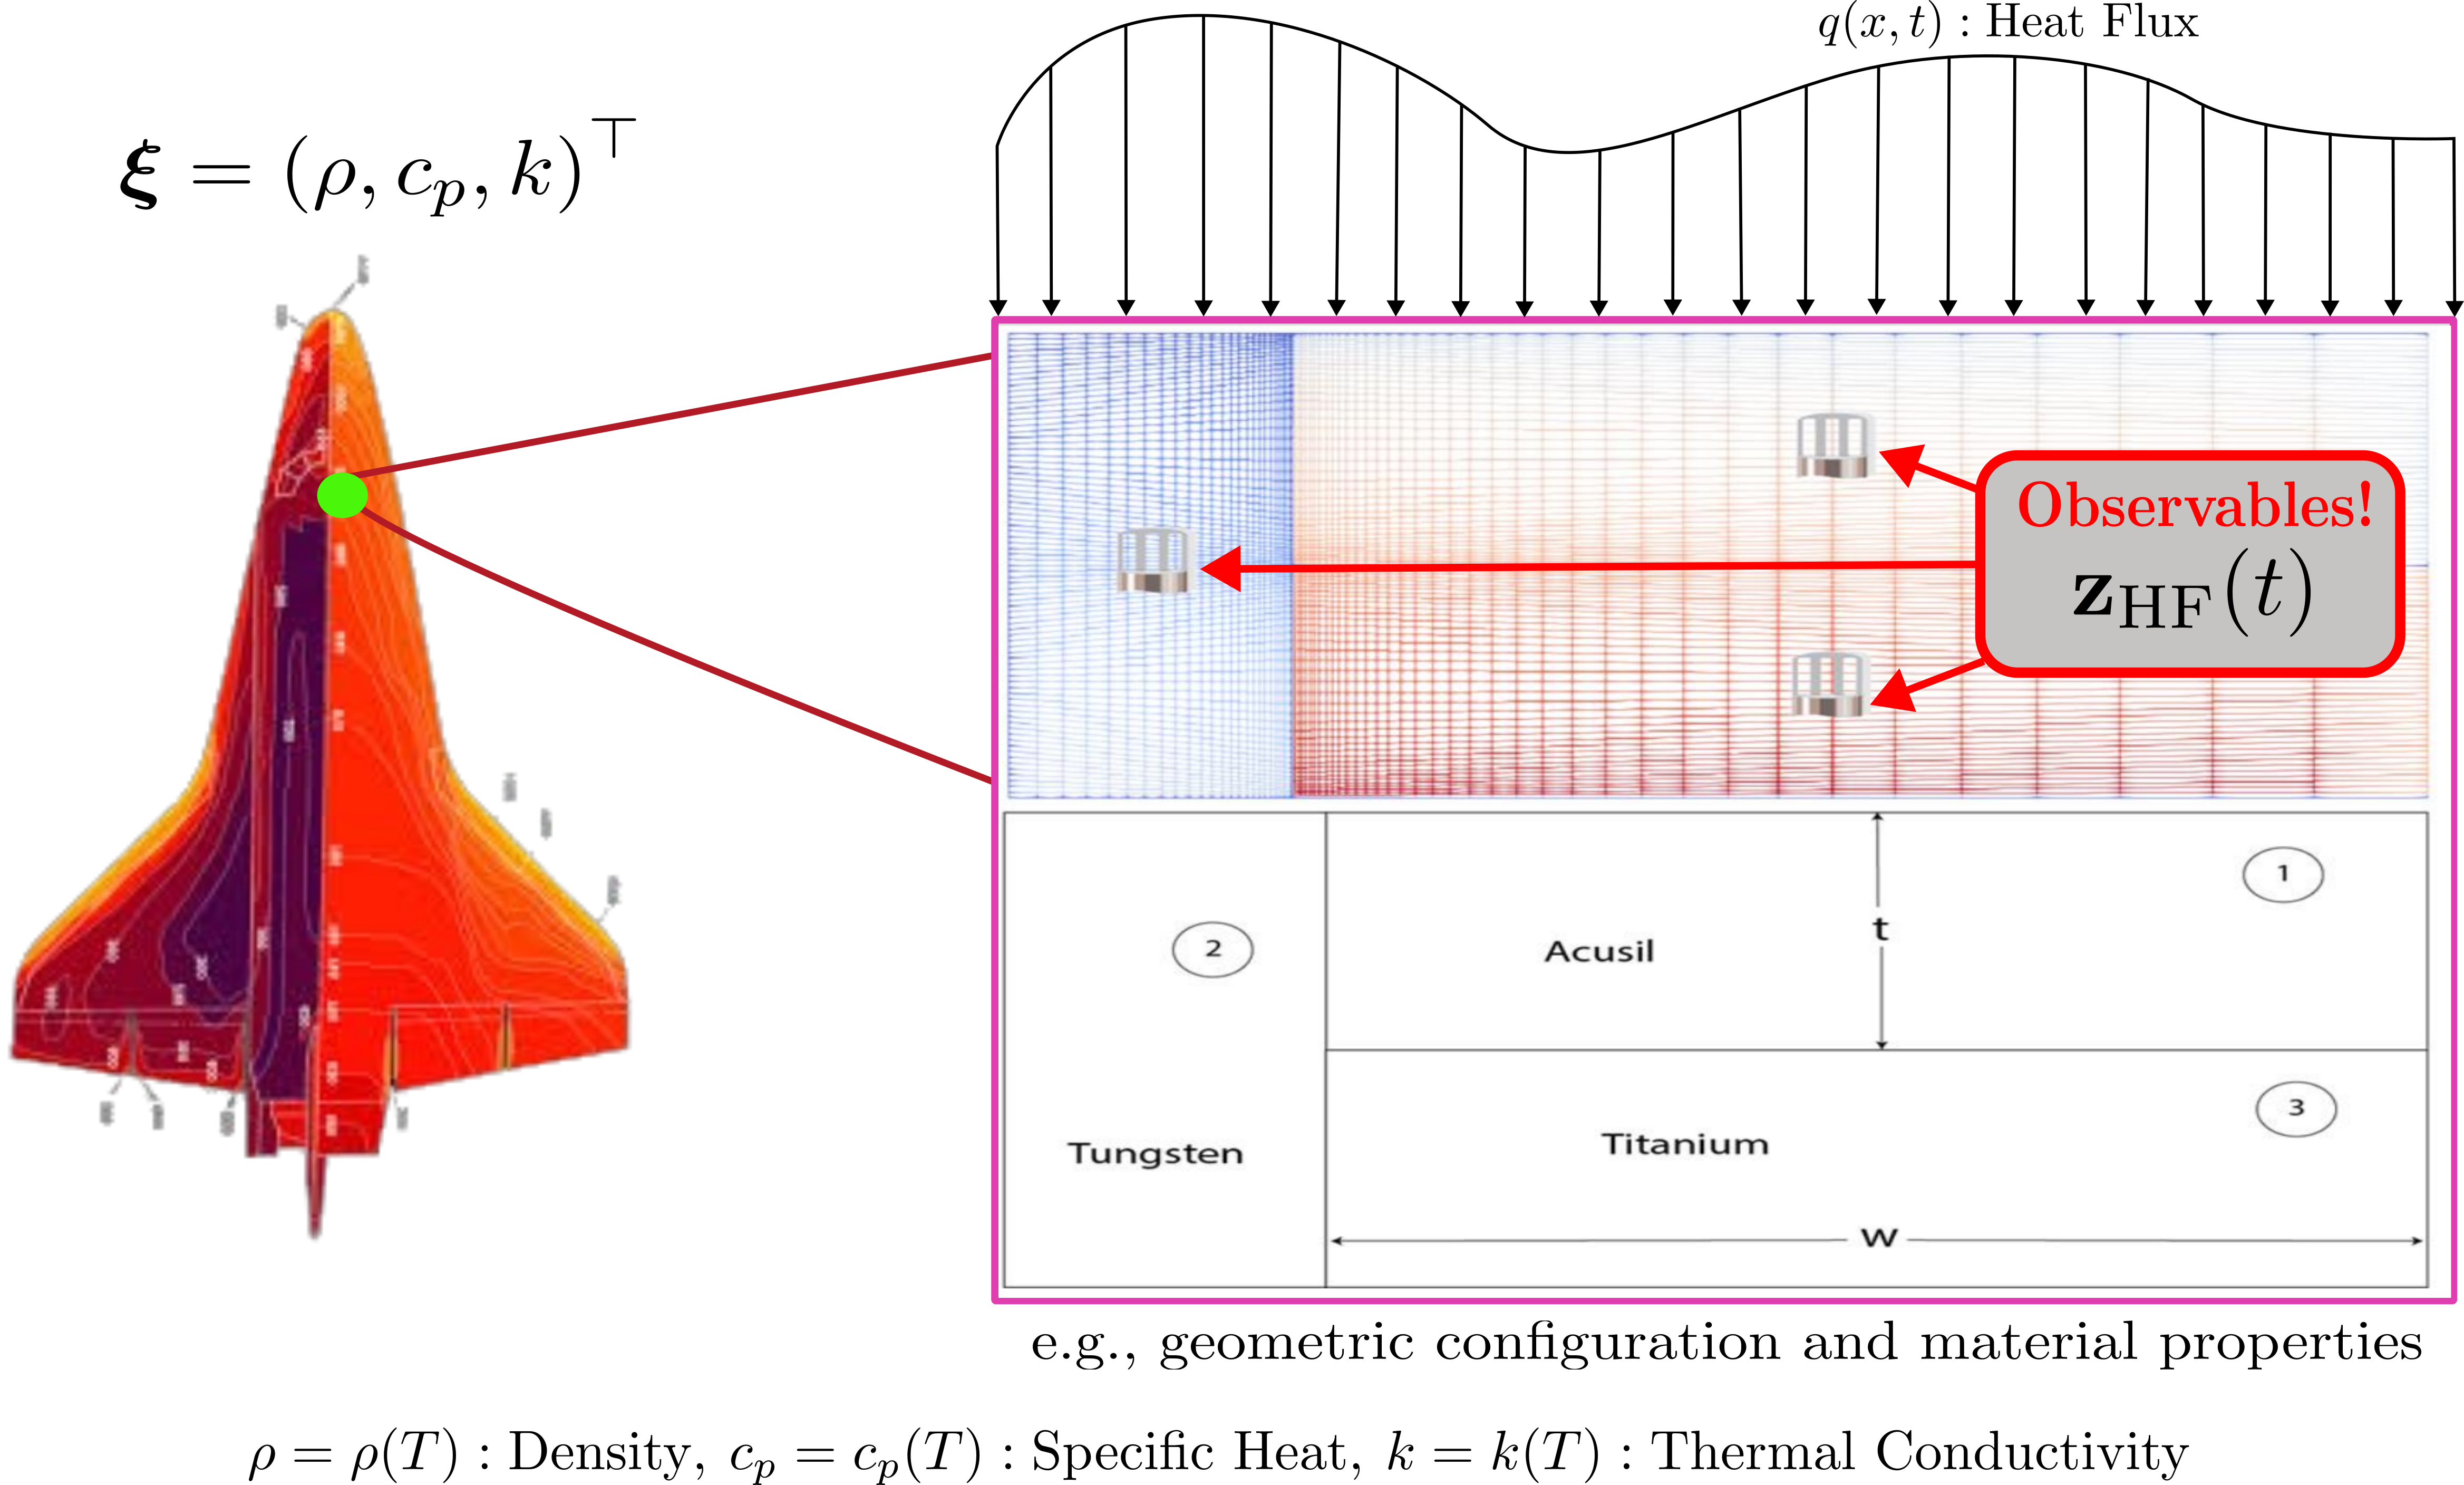
\includegraphics[width=0.9\textwidth]{../figs/pirom/tps.png}
            \end{figure}
        \end{column}}
        \hspace*{-0.4in}
        \begin{column}{0.38\textwidth}
            \visible<3->{
            \begin{graybox}{Parametrization}
                \visible<4->{
                Boundary conditions,
                \begin{align*}
                    \vxi_{\text{BC}} &= \left(\xi_0, \xi_1, \xi_2\right)^\top\\
                    q(x,t;\vxi_{\text{BC}}) &= q_1(x;\vxi_{\text{BC}})q_2(t;\vxi_{\text{BC}})    
                \end{align*}}
                \visible<5->{
                Material properties,
                \begin{align*}
                    \vxi_{\text{M}} &= \left(\alpha_0, \alpha_1, \alpha_2\right)^\top\\
                    m(T;\vxi_{\text{M}}) &= m^{(n)}(T) + m^{(p)}(T;\vxi_{\text{M}})
                \end{align*}}
            \end{graybox}}
        \end{column}
    \end{columns}
\end{frame}

\begin{frame}{Addressing the ITM: Learning the Hidden Dynamics}
    \footnotesize
    \visible<1->{
    We want to \textbf{extrapolate} to unseen boundary conditions and material properties,}
    \only<2>{
        \begin{figure}
            \centering
            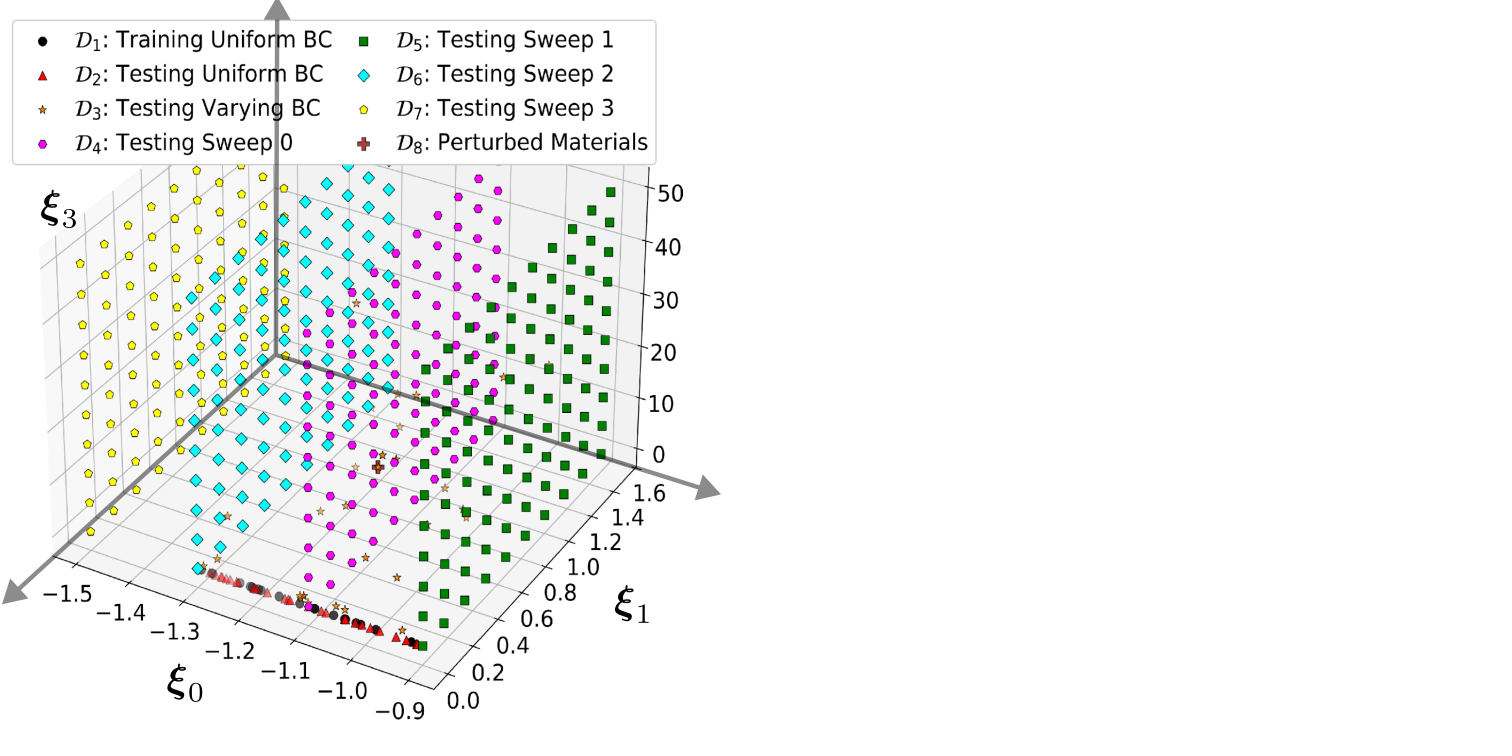
\includegraphics[width=0.8\textwidth]{../figs/pirom/tps_data_1.png}
        \end{figure}}
    \only<3>{
        \begin{figure}
            \centering
            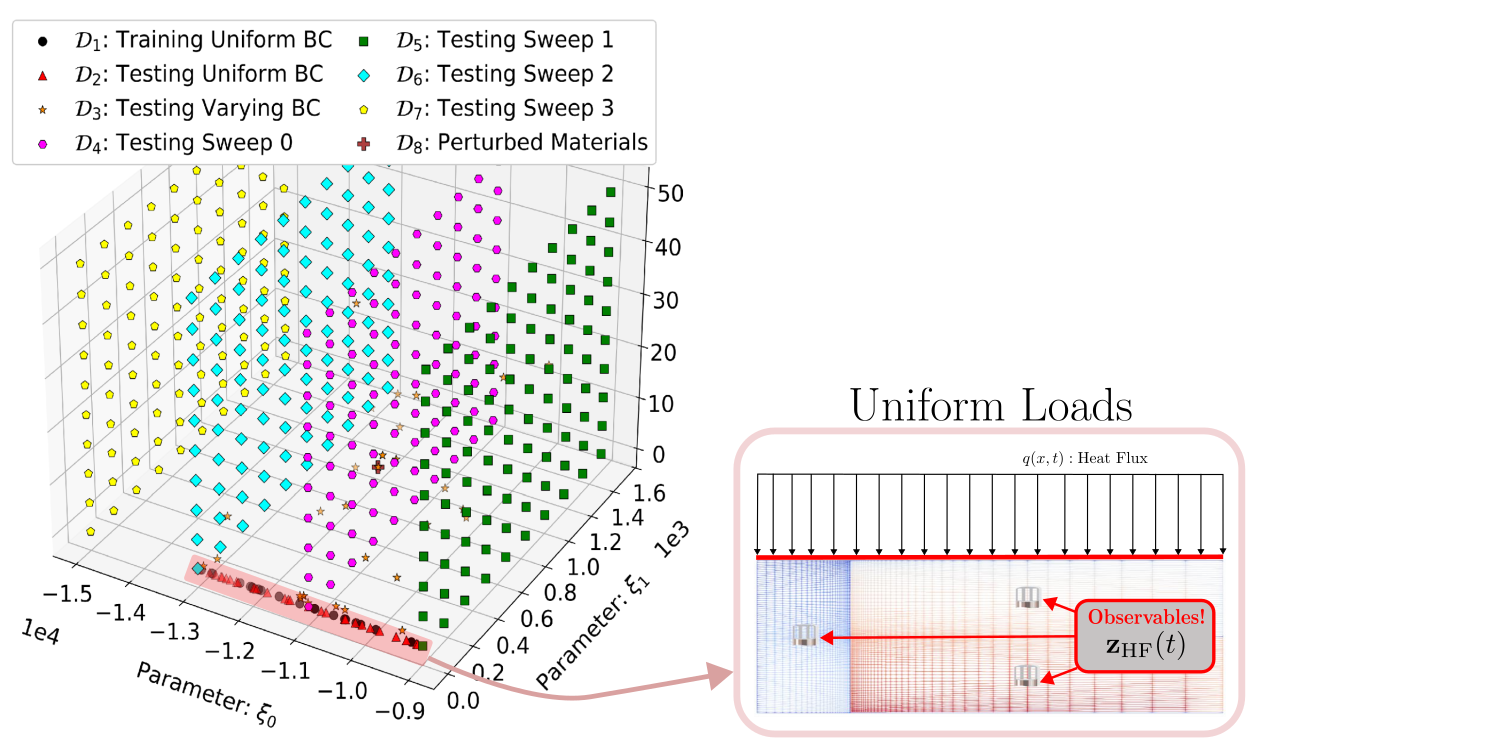
\includegraphics[width=0.8\textwidth]{../figs/pirom/tps_data_2.png}
        \end{figure}}
    \only<4>{
        \begin{figure}
            \centering
            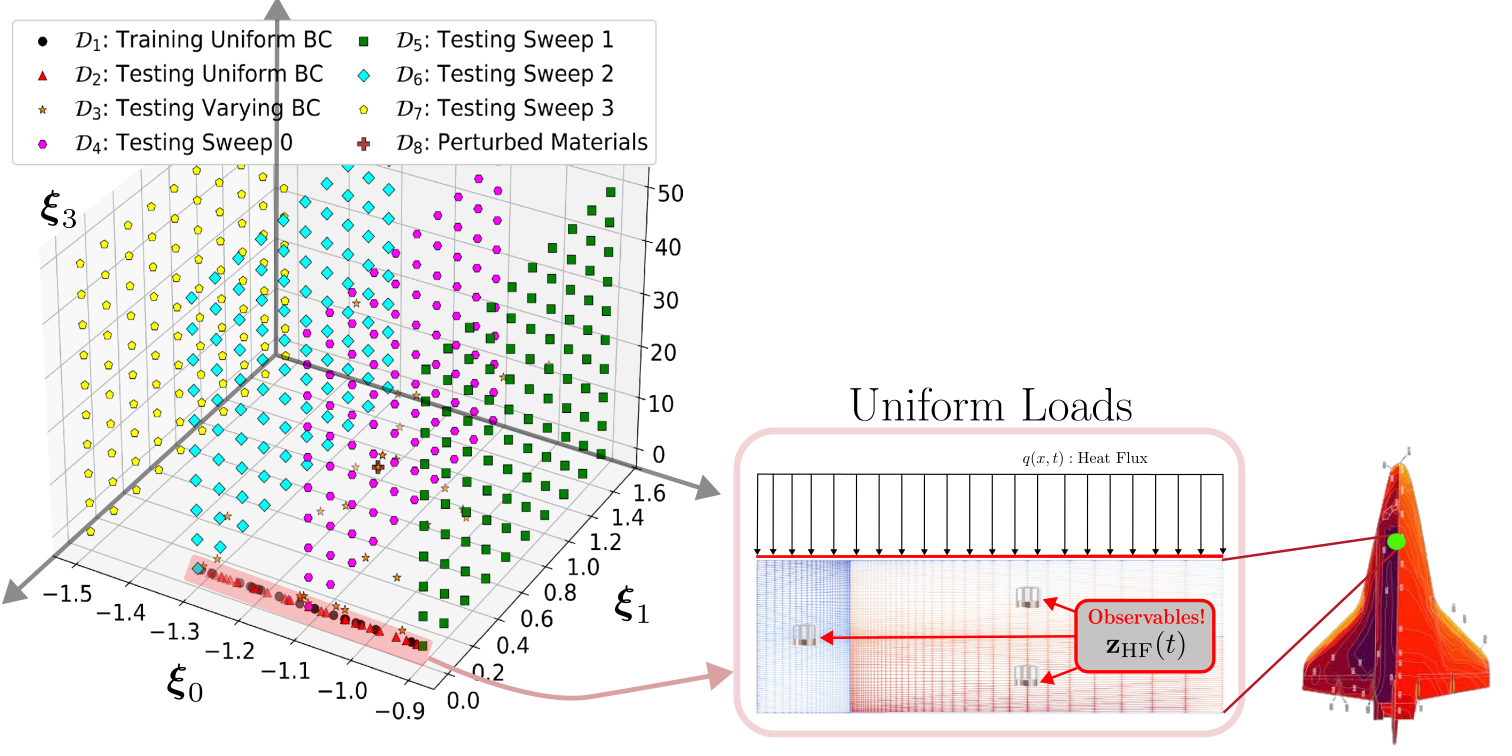
\includegraphics[width=0.8\textwidth]{../figs/pirom/tps_data_3.png}
        \end{figure}}
    \only<5>{
        \begin{figure}
            \centering
            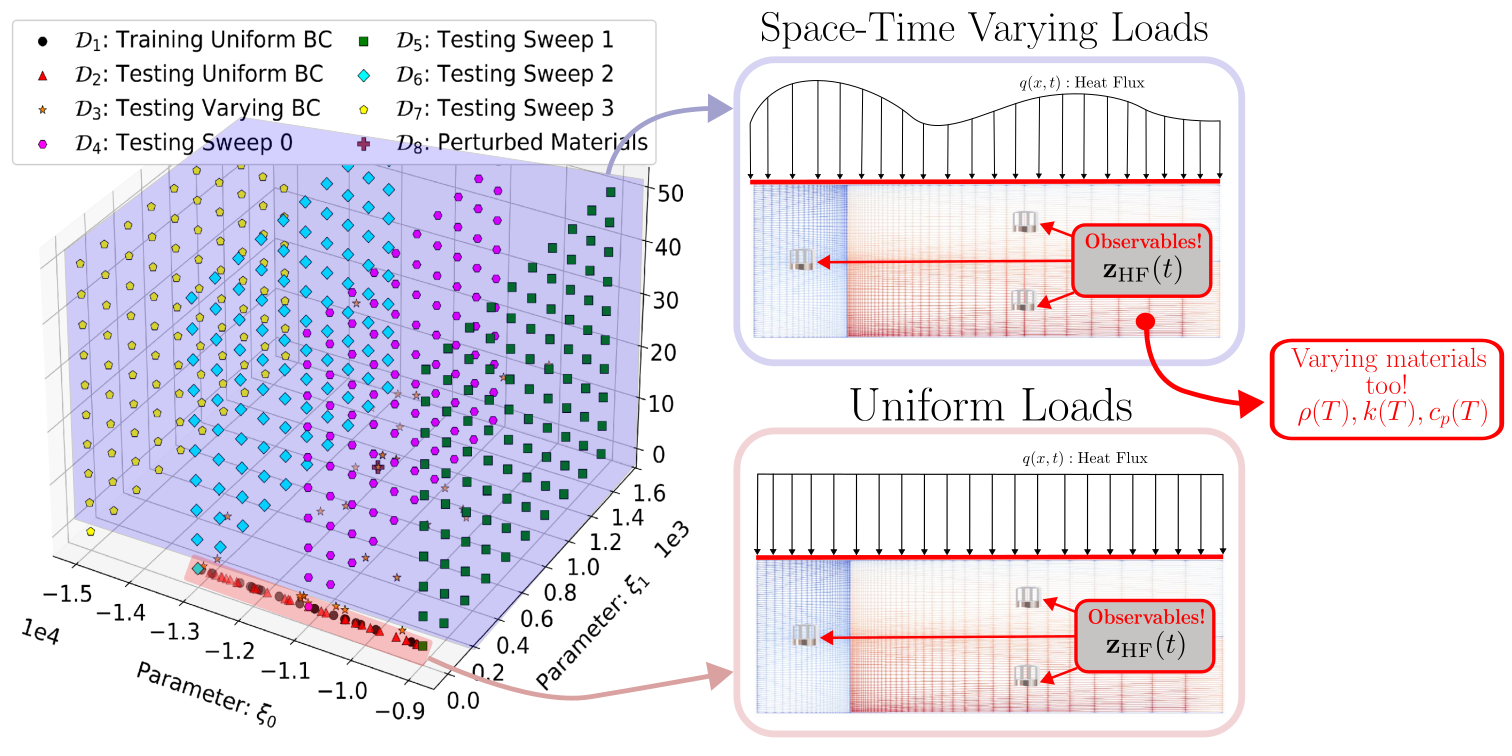
\includegraphics[width=0.8\textwidth]{../figs/pirom/tps_data_4.png}
        \end{figure}}
\end{frame}

\begin{frame}{Addressing the ITM: Results and Analysis}
    \footnotesize
    \visible<1->{\textbf{Quantify} the impossible trinity of modeling (ITM),}
    \vspace*{-0.05in}
    \begin{columns}
        \visible<2->{
        \begin{column}{0.4\textwidth}
            \begin{figure}
                \centering
                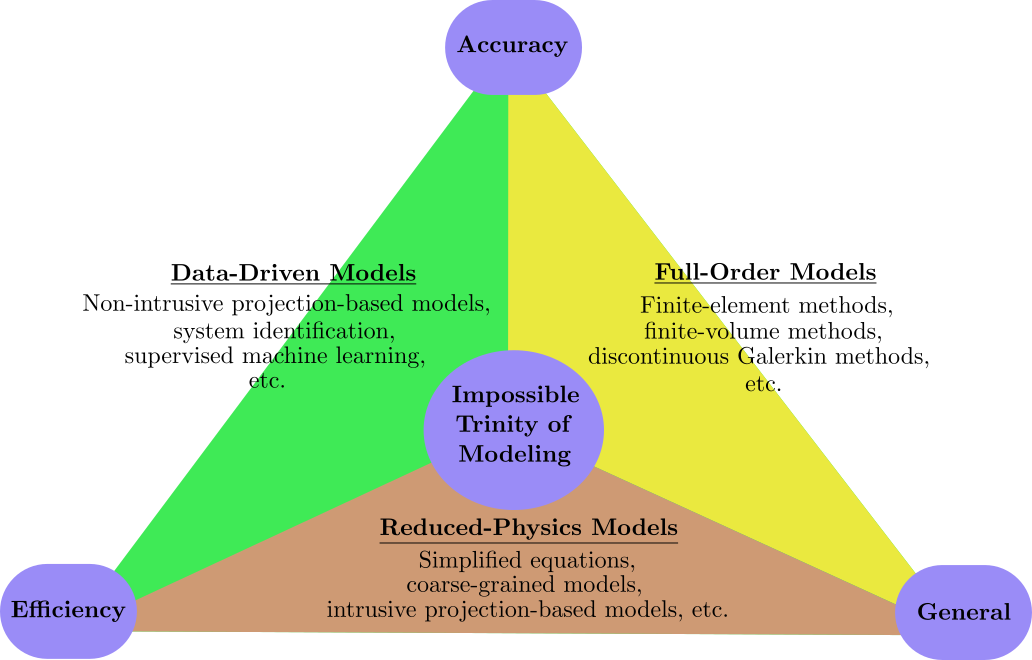
\includegraphics[width=0.9\textwidth]{../figs/introduction/itm.png}
            \end{figure}}
        \end{column}
        \vspace*{-0.1in}
        \begin{column}{0.6\textwidth}
            \centering
            \begin{itemize}
                \visible<3->{
                \item \textbf{Accuracy}: normalized root mean square error (NRMSE),
                \begin{equation*}
                    e_u^{(l)} = \frac{1}{\Delta z_{u,\text{HF}}^{(l)}}\sqrt{\frac{1}{p}\sum_{k=0}^{p-1}\left(z_{u,\text{HF}}^{(l)}(t_k) - z_{u,\text{ROM}}^{(l)}(t_k)\right)^2}
                \end{equation*}}
                \visible<4->{
                \item \textbf{Efficiency}: \textcolor{blue}{acceleration} ($\mathcal{A}$) and \textcolor{red}{overhead} ($\mathcal{O}$) factor,
                \begin{equation*}
                    \mathcal{A} = \frac{\mathcal{T}^{\text{predict}}_{\text{HF}}(\mathcal{D})}{\mathcal{T}^{\text{predict}}_{\text{ROM}}(\mathcal{D})},\quad \mathcal{O} = \frac{\mathcal{T}^{\text{train}}_{\text{ROM}}(\cD)}{\mathcal{T}^{\text{predict}}_{\text{HF}}(\cD)}
                \end{equation*}}
                \visible<5->{
                \item \textbf{Generalizability}: unseen BCs and materials,
                \begin{equation*}
                    \text{(\textcolor{red}{difficult for ROMs with sparse training data!})}
                \end{equation*}}
            \end{itemize}
        \end{column}
    \end{columns}
    \vspace{-0.28in}
    \begin{center}
        \tiny $\mathcal{T}_{\text{HF}}$: FOM wall-clock time, $\mathcal{T}_{\text{ROM}}$: ROM wall-clock time, $\Delta z_{i,\text{HF}}^{(l)}$: range of HF observables in trajectory $l$, $p$: number of time points, $\mathcal{D}$: dataset
    \end{center}
\end{frame}

\begin{frame}{Addressing the ITM: Results and Analysis}
    \footnotesize
    \visible<1->{Compare the performance of PIROM vs \textbf{SoTA SciML methods},}
    \hspace*{-0.5in}
    \only<2>{
    \begin{figure}
        \vspace*{-0.1in}
        \centering
        
\includegraphics[width=1.05\textwidth]{../figs/pirom/performance_1.png}
    \end{figure}}
    \only<3>{
    \begin{figure}
        \vspace*{-0.1in}
        \centering
        
\includegraphics[width=1.05\textwidth]{../figs/pirom/performance_2.png}
    \end{figure}}
    \only<4>{
    \begin{figure}
        \vspace*{-0.1in}
        \centering
        
\includegraphics[width=1.05\textwidth]{../figs/pirom/performance_3.png}
    \end{figure}}
    \only<5>{
    \begin{figure}
        \vspace*{-0.1in}
        \centering
        
\includegraphics[width=1.05\textwidth]{../figs/pirom/performance_4.png}
    \end{figure}}
    \only<6>{
    \begin{figure}
        \vspace*{-0.1in}
        \centering
        
\includegraphics[width=1.05\textwidth]{../figs/pirom/performance_5.png}
    \end{figure}}
    \visible<2->{
    \begin{center}
        {\tiny NODE: neural ordinary differential equations, OpInf: operator inference, NRMSE: normalized root mean square error, NN: neural network}
    \end{center}}
\end{frame}

\begin{frame}{Addressing the ITM: Results and Analysis}
    \footnotesize
    \begin{columns}
        \visible<1->{
        \begin{column}{0.4\textwidth}
            \centering
            \textbf{Is the ITM solved?}
            \begin{figure}
                \centering
                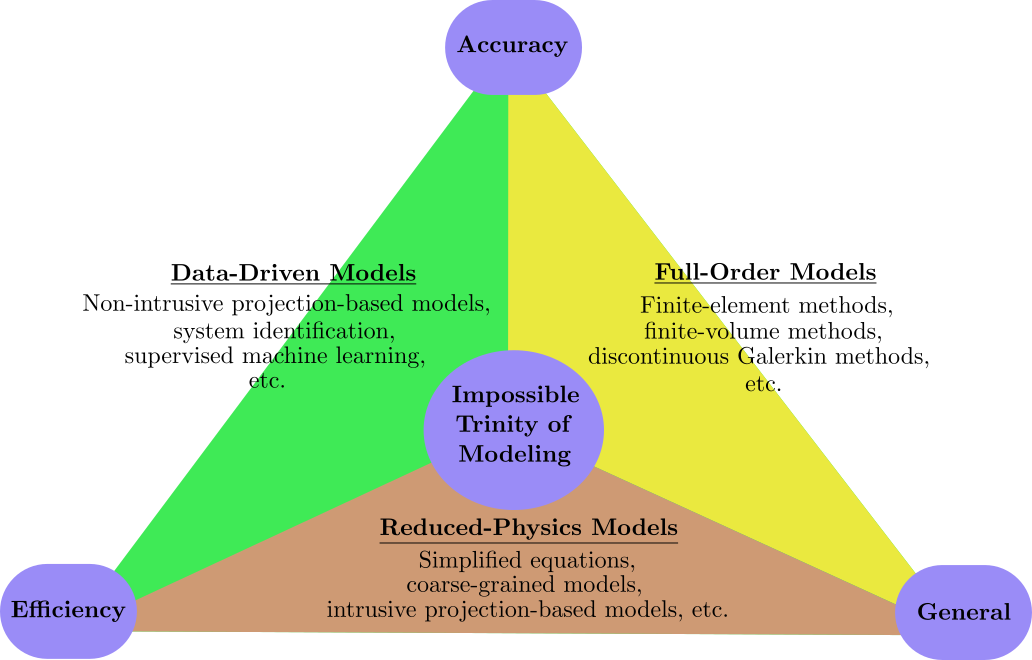
\includegraphics[width=0.9\textwidth]{../figs/introduction/itm.png}
            \end{figure}
        \end{column}}
        \begin{column}{0.7\textwidth}
            \centering
            \begin{itemize}
                \item<2-> \textbf{Accuracy}: comparable to FOMs (NRMSE $<1\%$),
                \item<3-> \textbf{Efficiency}: two-to-three orders of magnitude faster than FOMs,
                \item<6-> \colorbox{green!30}{\textbf{Generalizability}}:
                \begin{itemize}
                    \item<7-> \colorbox{green!30}{\textbf{Dimensions}: un-seen loading conditions},
                    \item<8-> \colorbox{green!30}{\textbf{Physics}: un-seen material properties} 
                \end{itemize}
                \visible<9->{
                \item \textbf{What about training efficiency?}}
                \begin{itemize}
                    \item<10-> \textbf{Overhead} is \colorbox{red!30}{$\approx$ 4 hrs in 3 CPUs} (similar to NODE),
                    \item<12-> therefore, we need to explore \colorbox{red!30}{other training approaches!}
                \end{itemize}
            \end{itemize}
        \end{column}
    \end{columns}
    \visible<2->{
    \begin{tikzpicture}[remember picture, overlay]
        \node[anchor=north west, xshift=2.29cm, yshift=-2.8cm] at (current page.north west) {
\includegraphics[width=0.1\textwidth]{../figs/pirom/checkmark.png}};
    \end{tikzpicture}}
    \visible<3->{
    \begin{tikzpicture}[remember picture, overlay]
        \node[anchor=north west, xshift=0.1cm, yshift=-5.8cm] at (current page.north west) {
\includegraphics[width=0.08\textwidth]{../figs/pirom/checkmark.png}};
    \end{tikzpicture}}
    \visible<6->{
    \begin{tikzpicture}[remember picture, overlay]
        \node[anchor=north west, xshift=4.45cm, yshift=-5.6cm] at (current page.north west) {
\includegraphics[width=0.1\textwidth]{../figs/pirom/checkmark.png}};
    \end{tikzpicture}}
\end{frame}